\chapter{Background}

% You should provide enough background to the reader 
% for them to understand what the project is all about, 
% and what is the relevant prior work.
% Examiners like to know that you have done the 
% appropriate background research and it is important 
% that you review either what has been done previously 
% to tackle related problems, or perhaps what other 
% products exist related to your deliverable. Clear 
% references are important here, and much of this 
% section will typically already have been written in your 
% Interim Report. You may use feedback from that 
% report to improve what you write in your Final Report, 
% and should note that self-plagiarism between the two 
% reports is not possible, so no citation is needed of 
% your own earlier writing.

%  What does the reader need to know in order 
% to understand the rest of the report? What 
% problem are you solving?
%  Why is this problem interesting or worthwhile 
% to solve?
%  Who cares if you solve it?
%  How does this relate to other work in this 
% area?
%  What work does it build on?
%  For 'research-style' projects involving the 
% design and analysis of specific algorithms 
% there is a large amount of relevant 
% background both of general theory, and very 
% specific to the algorithm you investigate. 
% Supervisors will help you to see what is most 
% important here, but the general rule is that 
% you must both provide overall context and 
% note work close to what you do that 
% influences your work or is in some way 
% comparable to your work.

This chapter outlines background information required for understanding the basis for the project. The theory and literature serves to outline the main concepts used for neuromorphic SLAM, as well as to reveal gaps in existing research that require solidifying.

\section{Event Cameras}

Event based cameras can be described as `bio-inspired sensors that differ from conventional frame cameras: Instead of capturing images at a fixed rate, they asynchronously measure per-pixel brightness changes, and output a stream of events that encode the time, location and sign of the brightness changes' \cite{EventBasedVisionASurvery}.

\subsection{Benefits}
Event-based cameras are purported to provide a number of benefits including, but not limited to;

\begin{itemize}
      \item \textbf{Very high temporal resolution}

            The reason for this is that whereas frame-based cameras have a certain frame-rate, event-based cameras do not have this limitation, meaning the "blind time" between frames is eliminated. The reason for this is that the function of a frame-based camera is dependent on the global shutter to capture the light at a particular instant, whereas event-based cameras can be thought of as having individual shutters for each pixel that are shut whenever an even occurs.
      \item \textbf{High dynamic range}

            The reason for this is again the fact that each pixel has its own individual shutter, but as well as this they all use a logarithmic scale, meaning they function well from very bright to very dim environments as well as fast shifts between the two.
      \item \textbf{Low power consumption}
      \item \textbf{High pixel bandwidth}

            Each pixel can capture events at the rate of ~kHz. This has the effect of reducing blur since there is a very high temporal resolution to begin with. This makes the system very responsive and therefore ideal for real-time systems.
      \item \textbf{Efficient Encoding}

            Since events are asynchronous and spatially sparse (i.e there are mainly 0 values in the matrix), the encoding is very efficient, as opposed to frame-based cameras that produce data that is very spatially dense.
\end{itemize}

The above benefits are very persuasive reasons to adopt neuromorphic cameras in many different applications. It is conceivable that if algorithms can make use of these benefits (since most classical algorithms play to the strengths of the data generated by frame-based cameras), real-time systems could be completely revolutionised.

\subsection{Function}
Event-based cameras differ from frame based cameras fundamentally, in that they do not rely on a global shutter closing at regular intervals to record information of a scene. Instead each pixel closes whenever it detects an 'event' occurring. The way to detects such events are dictated by the `event generation model'\cite{EventBasedVisionASurvery}.

Each pixel responds to changes in its log photo-current ($ L = log(I) $, where $I$ is the perceived brightness), giving the system a very high dynamic range. A recorded event '$ k $' has the format $ e_k = (\boldsymbol{\mathbf{x}}_k, t_l, p_k ) $. THis is known as the Address Event Representation (AER). The first value is the spacial location of the event ($ \boldsymbol{\mathbf{x}}_k = (x_k, y_k)^\top $), the second value $ t_k $ is the temporal location, and the final value $ p_k \in {1, -1} $ indicates the polarity of the event (i.e in which direction the brightness gradient was changing). The brightness increment between two events at the same pixel is given by the equation $ \Delta L(\boldsymbol{\mathbf{x}}_k, t_k) = L(\boldsymbol{\mathbf{x}}_k, t_k) - L(\boldsymbol{\mathbf{x}}_k, t_k - \Delta t_k) $. In a perfect (noise free) environment an event is fired whenever the brightness increment reaches a temporal contrast threshold given by the equation $ \Delta L(\boldsymbol{\mathbf{x}}_k, t_k) = p_k C $ ($ C > 0 $). It should be noted that the value of $ C $ could be variable and therefore different for $ p_k = \pm 1 $.

Additionally, we can approximate the temporal derivative of a pixels brightness by utilising the following Taylor expansion:

$$ \Delta L(\boldsymbol{\mathbf{x}}_k, t_k) \approx \frac{\delta L}{\delta t}(\boldsymbol{\mathbf{x}}_k, t_k)\Delta t_k $$
$$ \frac{\delta L}{\delta t}(\boldsymbol{\mathbf{x}}_k, t_k) \approx \frac{\Delta L(\boldsymbol{\mathbf{x}}_k, t_k)}{\Delta t_k} = \frac{p_k C}{\Delta t_k} $$

The above approximation, however, is only true under the assumption that $ \Delta t_k $ is exceedingly small. Since unlike frame-based cameras we do not measure absolute brightness, this is an indirect way of measuring and keeping track of the brightness within the frame.

\autoref{fig:davis_camera} shows the basic functionality of an event based camera. \textbf{(a)} is the simplified circuit diagram of the DAVIS pixel, which in \textbf{(b)} is used to convert light into events (shown in real life in images \textbf{(c)} and \textbf{(d)}). \textbf{(e)} shows how this setup would view a white square rotating on a black disk. It is a stream of events going from the past in green to the present in red. These events can then be seen overlaid on a natural scene in \textbf{(f)}.

\begin{figure}[htb]
      \centering
      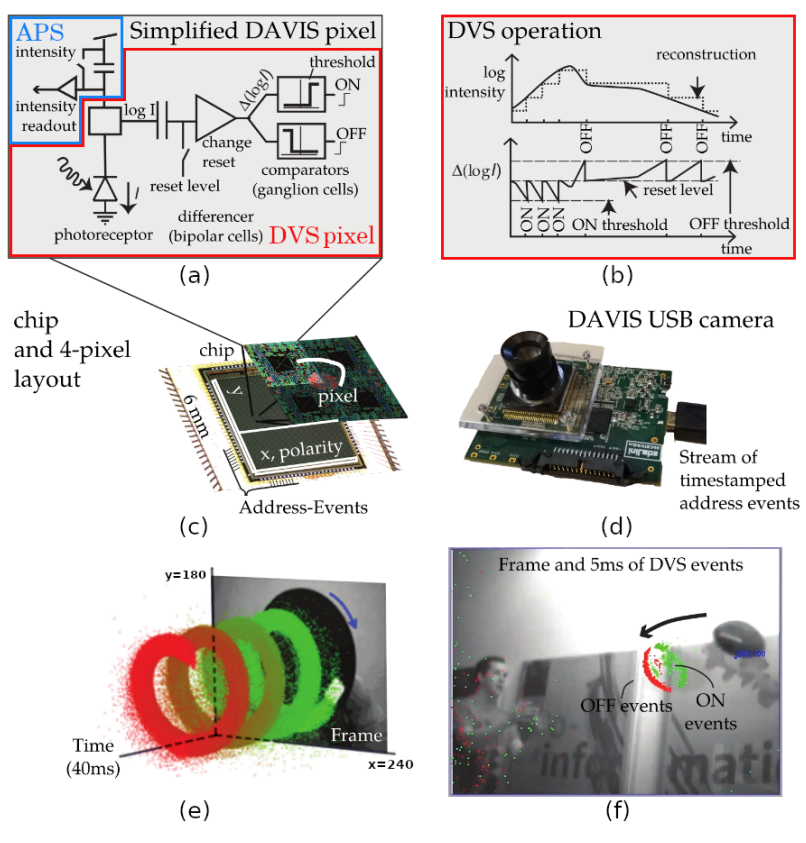
\includegraphics[width=0.5\textwidth]{background/images/davis_camera.png}
      \caption{Summary of DAVIS event based camera\cite{EventBasedVisionASurvery}}
      \label{fig:davis_camera}
\end{figure}

\subsection{Optic-flow Methods}

More classic computer vision techniques using optic-flow constraints can now be utilised to characterise the events detected by pixels. In frame-based systems, optic flow methods create a flow-field that describe the displacement vector (signifying direction and magnitude of movement) for each pixel in the frame. A core constraint in this derivation is that the intensity of a local time-varying image region is constant under motion (for at least a short amount of time)\cite{GenerativeEventModel}.

\color{red} NEED TO READ AND UNDERSTAND WHY THE FOLLOWING IS TRUE \cite{GenerativeEventModel} \cite{EventBasedVisionASurvery} \color{black}

$$ \Delta L \approx -\nabla L \cdot v \Delta t_k $$

\section{Spiking Neural Networks and Neural Heterogeneity}

Above are very persuasive reasons for utilising neuromorphic systems, but there still many challenges posed when attempting to do so. For example, each pixel only responds to brightness change, but the problem is that such a change could be a result of not only scene changes, but also the position of the camera within the scene. For this reason most neuromorphic systems have currently been limited to stationary cameras. As well as this the system is especially prone to stochastic noise, due to inherent shot noise in photons and from transistor circuit noise \cite{EventBasedVisionASurvery}. In order to tackle such issues, it is useful to look at existing examples of spiking neural systems, such as biological brain with neurons working based on a spiking function. It is known that the brain is heterogeneous on every scale, in the past this was though to be simply a by-product of noisy processes, but more recently it can be shown that by evolving our largely homogeneous Spiking Neural Networks (SNNs), we can create more stable and robust systems \cite{NeuralHetroPromRobLearn}.

The foundations of SNNs are in computational neuroscience. The mechanisms of neurons in the brain are the inspiration behind creating artificial neural networks with neurons that spike in the same way. Neurons in an a typical Artificial Neural Network (ANN) have a weight, bias and activation function. this means the output of the neuron can be specified as:

$$ y = \theta(\sum^n_{j=1}w_jx_j-u_j) $$

This model was inspired by the biological neuron model shown in \autoref{fig:biological_neuron}. The function of the neuron is similar in that it produces an output based on a function of the input stream, but he form of this output is in the form of a `spike' rather than a continuous function. The $ \Sigma $ shown in the diagram is actually the integration of all excitory and inhibitory input signals to the dendrites within the soma of the neuron. We can see that the electric potential of the neuron needs to exceed a certain threshold in order for the output of the neuron to be a spike. Spiking neural networks use a similar model of neurons in order to leverage the aforementioned benefits of neural heterogeneity.

\begin{figure}[htb]
      \centering
      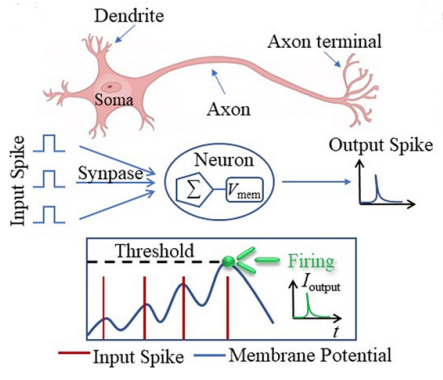
\includegraphics[width=0.4\textwidth]{background/images/biological_neuron.png}
      \caption{Diagram of structure and function of a biological neuron \cite{BiologicalNeuronModel}}
      \label{fig:biological_neuron}
\end{figure}

\color{red} NEED TO READ EVENT PAPER TO SEE THEIR APPROACH TO STOCHASTIC NOISE \cite{EventBasedVisionASurvery}. ALSO READ PAPER\cite{NeuralHetroPromRobLearn} TO INCLUDE IMAGE OF AND EXPLANATION OF BRAIN NEURONS \color{black}

\section{Existing Algorithms for Event Analysis}

For SLAM and pose estimation the problem again is that classical systems heavily rely on the structure of conventional cameras, and so there needs to be a radical paradigm shift in order to take events as inputs instead. The reason for this is that their function depends on iterative changes to the location probabilities using inputs, for which spiking inputs are ideal.

\subsection{Probabilistic Filters}

\subsubsection{Bayesian Inference}

Unlike most other previous systems, probabilistic filters such as Bayesian filters inherently work for the new scenario with event-based cameras. Bayes's theorem can be derived from simple probabilistic rules\cite{BayesLaw}. We know $P(X|Y) = \frac{P(X, Y}{P(Y)} $ and similarly $ P(Y|X) = \frac{P(Y, X)}{P(X)} $. Therefore we can re-arrange both to give $ P(X|Y)P(Y) = P(Y|X)P(X) $, since $ P(X, Y) = P(Y, X) $. Then from there formula for Bayesian inference can be trivially obtained:

$$ P(XZ) = P(Z|X)P(X) = P(X|Z)P(Z) $$
$$ P(X|Z) = \frac{P(Z|X)P(X)}{P(Z)}$$

In the above equations $ X $ is known as the prior (which is the assumed location of the camera) and $ Z $ is known as the posterior (which is the measurement taken by the sensor or camera). $P(Z|X) $ is known as the likelihood function, which indicates how likely it is to have received the particular reading given the assumed position.

\subsubsection{Monte-Carlo Localisation}

Now that we have the concept of Bayesian inference we can adapt it to create an efficient localisation algorithm. It includes initialising a number of particles that act as predictors of where in the map the camera is. We can now give the probability of a posterior camera position given a sensor reading.

The probability distribution $ P(X|X) $ is a continuous function, and so updating each of the posteriors for every value of $ X $ is a computationally difficult problem. We can instead break it up into smaller bins to alleviate this issue. When generating these particles we can represent the probability distribution, albeit at a lower granularity. The benefit of this is that even though we cannot see the full distribution the peaks (i.e. the locations the camera is most likely to be in) are very well defined.

Now we can use the above simplification to carry out the following steps:

\begin{enumerate}
      \item Randomly assign particle distribution across map
      \item Apply Bayes' law to measurement to update particle distribution

            Bayes' rule can be simplified to be:
            $$ w_{i_{x+1}} = P(z|x_{i_x}) \times x_{i_x} $$
            This can be done since the ignored multiplier on the right hand side will be normalised in the next step.
      \item Normalise particle weights

            Now the particles will have weights that no longer sum to 1, and so we need to normalise them again to follow the usual rules of probability:

            $$ w_{i_{x+1}} = \frac{w_i}{\sum^N_{i=1}w_i} $$
      \item Re-sample particle distribution

            We now need to create a new set of particles that all have the same weight ($ \frac{1}{N} $, but whose spacial distribution now reflects the probability density.
\end{enumerate}

\begin{figure}[htb]
      \centering
      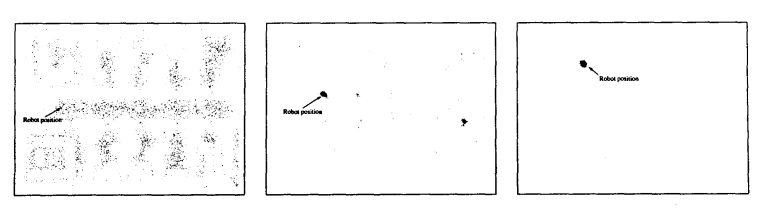
\includegraphics[width=\textwidth]{background/images/monte_carlo.png}
      \caption{Example of Monte-Carlo localisation\cite{MonteCarloLocalisation}}
      \label{fig:monte_carlo}
\end{figure}

\autoref{fig:monte_carlo} shows a typical example of the algorithm. The leftmost panel shows the random initialisation (or previous particle distribution), which then becomes the centrally shown distribution after one iteration. Since only one measurement is taken and the room is symmetrical it is possible that it could be in one of two location (hence the two dense clusters). After one more reading in the next iteration the algorithm is quickly able to narrow down the location of the robot. We can also see that any movement of the robot causes some noise to be added to the known robot location as we are estimating the location based on simple odometry using hardware such as wheel encoders to estimate the robots motion.

This algorithm, however, is classical and has therefore been mostly superseded by deep neural networks in most modern day applications. As well as this it is only applicable to localising the robot, whereas we want to be able to simultaneously map it. SLAM can be achieved using similar methods by identifying and moving around located points of interest and estimating their positions as well as the robots. These tasks have been efficiently solved by neural networks for classical frame based data, but there is still much ongoing research on how to do the same with spiking data.

\subsection{SLAM Algorithm}

The Monte-Carlo localisation technique is useful for estimating a vehicles position (i.e, its location and orientation) given a model (or map) of the environment surrounding it. Now we must do the pose estimation of a robot while simultaneously generating a map of its surroundings (as shown in \autoref{fig:slam_diagram}). It is clear from the diagram that the equipment is not perfect and in an idealised environment. There us uncertainty in both the robot position (since there is uncertainty in the robots odometry), and there is also uncertainty in the measurements the robot takes.

\begin{figure}[htb]
      \centering
      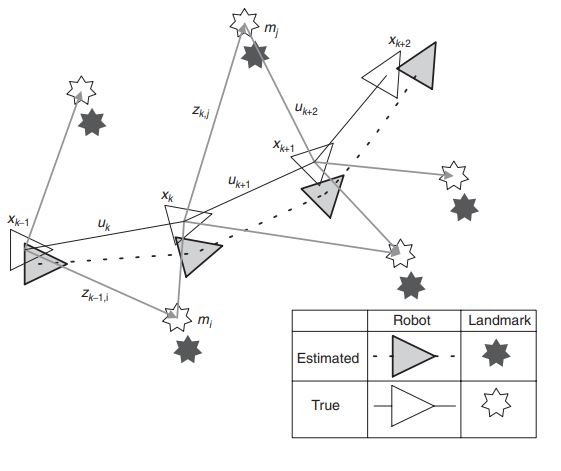
\includegraphics[width=0.4\textwidth]{background/images/slam_diagram.png}
      \caption{Diagram showing the fundamentals of the SLAM problem\cite{BasicSlam}}
      \label{fig:slam_diagram}
\end{figure}

There are two main branches of SLAM algorithms; filtering methods and smoothing methods. The former includes methods such as the Extended Kalman Filter (EKF) and particle filtering (similar to the Monte-Carlo filtering explained earlier). With these methods the state is estimated iteratively on the job as latest measurements are input into the system. The latter uses the set of complete measurements to estimate the full trajectory of a robot. Pose (or factor) graph optimisation is one such smoothing method that has become exceedingly popular in modern-day SLAM solutions.

\begin{figure}[htb]
      \centering
      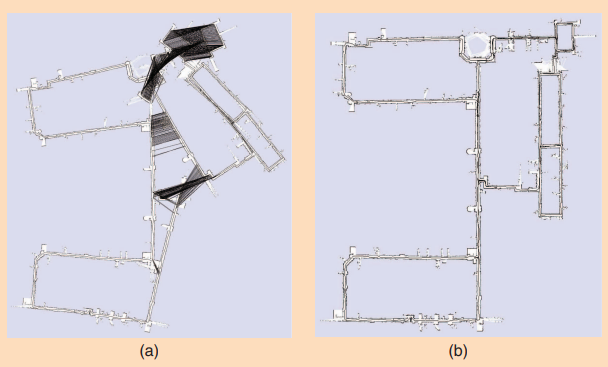
\includegraphics[width=0.4\textwidth]{background/images/slam_graph_optimisation.png}
      \caption{Diagram showing loop closer and optimisation steps of SLAM pose graph optimisation technique\cite{PoseGraphOptimisation}}
      \label{fig:slam_graph_optimisation}
\end{figure}

The pose graph optimisation technique relies on memorising the robots relative position and the readings it took in that position. For example we can see a possible robot trajectory in \ref{fig:slam_diagram}. The robot and its new relative positions are all nodes of the graph and are connected by edges. Whenever a new node is created in the graph, a reading is also taken and stored. Then whenever a new node is visited it is compared with previously stored readings, and if there is a reading that is similar to a very high degree, `loop closure' can take place. In essence this means that the robot is now visiting a location it has already visited, and so the nodes can be joined together. Then once each the loop has been established we need to optimise the graph so that each edge (and therefore node) is at its most likely position relative to the other edges. The way this is done is that each edge of the graph has a relative certainty associated with it, and this certainty dictates how flexible that particular edge is in the optimisation process. Once the loop has been closed the edges are moved such that the overall certainty of the graph is maximised. Once this is complete the readings can be stitched together to form a map of the environment, and the location of the robot within it is very well defined. This process can be seen clearly in \autoref{fig:slam_graph_optimisation}, where in \textbf{(a)} loop closure takes places, and \textbf{(b)} shows the map created after the subsequent optimisation phase. The maps are created using `binary occupancy grids' or `probabilistic grids'. The former simply stores binary 1's and 0's on whether a particular section of the grid is occupied or not. The latter adapts this by having probabilities of occupancy for each section rather than just binary values.

\section{Existing Datasets}

There already exists many repositories of recorded neuromorphic data to get familiar with spiking data. In this section there are some examples of such datasets and a quick overview of their contents.

\subsection{Neuromorphic-MNIST and Other Neuromorphic Datasets}

This data-set is a spiking version of the original frame-based MNIST dataset \cite{MNIST}\cite{NMNIST}. The dataset is identical to the original MNIST dataset, which is a set of handwritten digits, in all ways (including scale, size and sample split) bar one - it was captured using an ATIS sensor mounted on a motorised pan-tilt unit. This sensor moved while viewing the MNIST examples on an external monitor.

For each item in the dataset there is a binary file which has a list of events. Each event is characterised by a 40 bit unsigned integer. The integer gives the following information of a particular event:

\begin{itemize}
      \item bit 39 - 32: X location (in pixels)
      \item bit 31 - 24: Y location (in pixels)
      \item bit 23: Polarity (0 for OFF, 1 for ON)
      \item bit 22 - 0: Timestamp (in microseconds)
\end{itemize}

An example of a visualisation of this data is shown in \autoref{fig:nmnist_spikes_visualisation}, where the image used from the MNIST dataset is on the right in part \textbf{(b)} and the resulting spikes from the event-based camera are shown on the left in \textbf{(a)}. Here `on events' are events where the intensity of a the particular pixel increased by an increment greater than a threshold and the `off events' are when the intensities decrease by a increment less than a threshold. The representation is clearly very different to the one given by a classical camera, and therefore the use of such data has to have a different approach to classical techniques.

\begin{figure}[htb]%
      \centering
      \subfloat[\centering]{{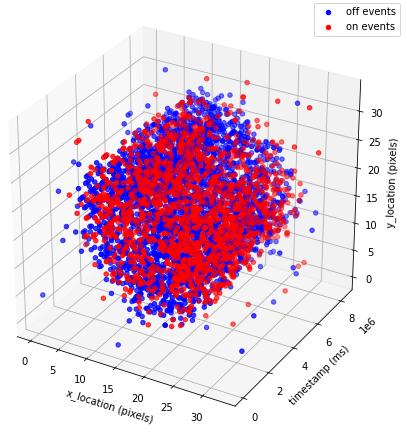
\includegraphics[width=0.35\textwidth]{background/images/nmnist_spikes_visualisation.png}}}%
      \qquad
      \subfloat[\centering]{{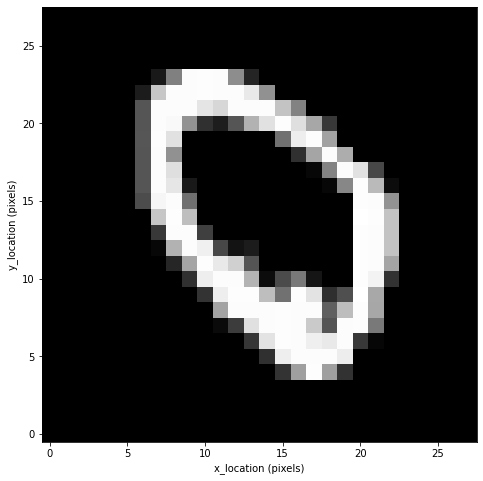
\includegraphics[width=0.35\textwidth]{background/images/mnist_matching_nmnist.png}}}%
      \caption{Visualisation of events from a single training sample from the NMNIST dataset}%
      \label{fig:nmnist_spikes_visualisation}%
\end{figure}

More examples of neuromorphic datasets include:

\begin{itemize}
      \item \textbf{DVS128}

            This dataset is a set of 11 hand gestures from 29 subjects under 3 illumination conditions. It was created to help create a real-time gesture recognition system that utilises the low power capabilities of frame-based cameras\cite{DVS128}.
      \item \textbf{Heridelberg Spiking Datasets}

            The Spiking Heidelberg datasets for spiking neural networks\cite{SpikingHeidelberg} are useful for realising that spiking data is useful for so many more applications than computer vision. This dataset is split into two; The Spiking Heidelberg Digits (SHD) dataset and the Spiking Speech Command (SSC) dataset. Both of these datasets are audio-based classification datasets for which input spikes and output labels are provided.
\end{itemize}

\subsection{Non-neuromorphic Datasets}

Other data-sets such as fashion MNIST could also be converted to spiking times by treating image intensities as input currents to model neurons, so that higher intensity pixels would lead to earlier spikes, and lower intensity to later spikes.

\section{Image Reconstruction Algorithms}

Image reconstruction has been implemented for event data using on the direct optimised versions of Convolutional Neural Networks (CNNs). An example of this is the network named 'U-net'\cite{UNET} which managed to reconstruct a video using 10M parameters to analyse events from an AER camera protocol. Recent work by Rebecq \textit{et al.} illustrates a novel network architecture that reconstructs a video from a stream of events \cite{spikingToVideo}. These methods are purported to allow the introduction of mainstream computer vision research to event cameras. \autoref{fig:spikes_to_video} shows an example of how converting spiking data to a video stream allows for use of classical computer vision algorithms.

\begin{figure}[htb]
      \centering
      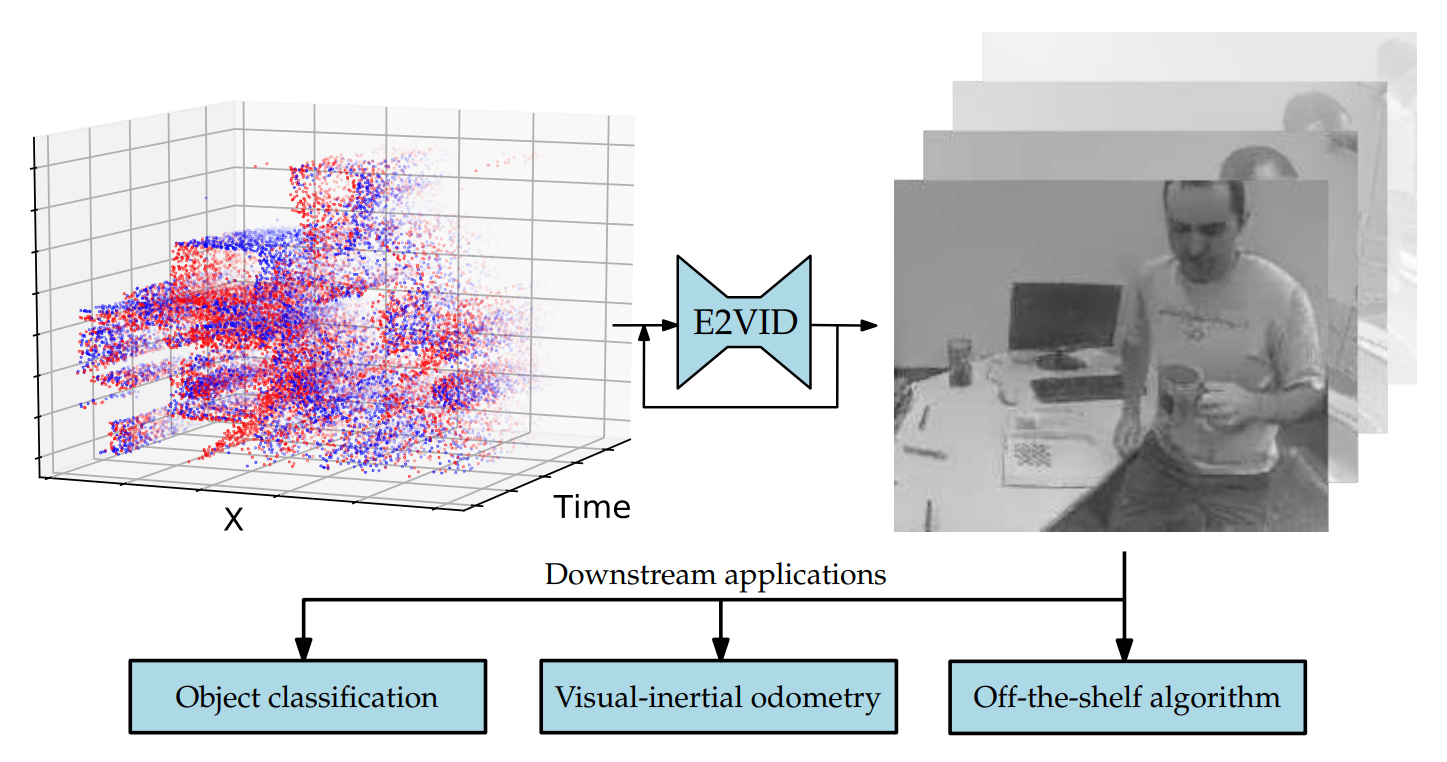
\includegraphics[width=0.7\textwidth]{background/images/spikes_to_video.png}
      \caption{Illustration of mapping of spiking data to video stream to apply off-the-shelf algorithms to\cite{spikingToVideo}}
      \label{fig:spikes_to_video}
\end{figure}

A naive approach would be take take each would be to take each event $ e_k = (\boldsymbol{\mathbf{x}}_k, t_l, p_k ) $ and assuming that the firing was due to the brightness change was due to a brightness change above a threshold $ \pm C $ which is a constant that could be set by the user. If this was the case events could be directly integrated to recover the intensity map of images. however, the value $ C $ in reality does not remain constant and is heavily dependent on other factors such as event rate, temperature, and sign of brightness change. The implementation outlined instead makes use of a Recurrent Neural Network (RNN), that takes as input sets of events within a spatio-temporal window. For example, a stream of events will be broken down into sequences given by $ \epsilon_i \: \forall i \in [0, N-1] $. Since each sequence is of fixed length $ N $ the framerate of the output video from the RNN is proportional to the event rate. \autoref{fig:spikes_to_video_rnn} shows demonstrates the functionality of such a network. Each event window $ \epsilon_k $ is converted to a 3D event tensor and passed into the network along with the last $ K $ constructed images to generate the latest iteration of the image. It is clear from this that each new image is constructed by fusing the previous K images with the new stream of events.

\begin{figure}[htb]
      \centering
      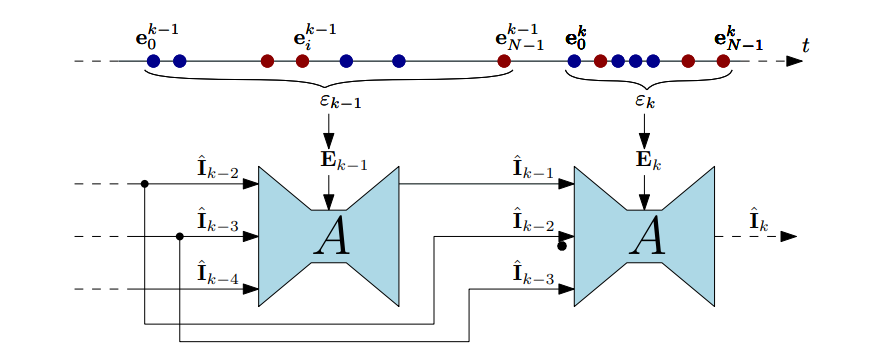
\includegraphics[width=0.6\textwidth]{background/images/spikes_to_video_rnn.png}
      \caption{Overview of RNN used to generate video from sets of events\cite{spikingToVideo}}
      \label{fig:spikes_to_video_rnn}
\end{figure}

\color{red} NEED TO EXPLAIN ARCHITECTURE PROPERLY\cite{spikingToVideo} \color{black}